\section{Распределения для связанных состояний CO$_2-$Ar}


Для нахождения распределений гамильтоновых переменных в связанных состояниях CO$_2-$Ar сформируем Марковскую цепь в подпространстве $H < 0$ фазового пространства $\Gamma$. Генерацию точек Марковской цепи также осуществим методом MH с некоторой модификацией.

\begin{algorithm}[!h]
\begin{algorithmic}[1]
		\caption{Scheme of modified Metropolis-Hastings algorithm} \label{bound}
\State Initialize $x^{(0)} \sim q(x)$
\State \textbf{for} iteration $i = 1, 2, \dots$ \textbf{do}
\State \quad Propose: $x^{cand} \sim q \lb x^{(i)} | x^{(i-1)} \rb$
\State \quad Calculate: $E^{cand} = H \lb x^{cand} \rb$ 
\State \quad \textbf{if} $E^{cand} > 0$ \textbf{then}
\State \qquad Reject the proposal: $x^{(i)} \gets x^{(i - 1)}$
\State \quad \textbf{else}
\State \qquad \textbf{continue}
\State \quad \textbf{end if}
\State \quad Acceptance probability:
\State \qquad $\alpha \lb x^{cand} | x^{(i-1)} \rb = \min \left\{ 1, \frac{q \lb x^{(i-1)} | x^{cand} \rb \pi \lb x^{(cand)} \rb }{ q \lb x^{cand} | x^{(i-1)} \rb \pi \lb x^{(i-1)} \rb} \right\}$
\State \quad $u \sim$ Uniform(u; 0, 1)
\State \quad \textbf{if} $u < \alpha$ \textbf{then}
\State \qquad Accept the proposal: $x^{(i)} \gets x^{cand}$
\State \quad \textbf{else}
\State \qquad Reject the proposal: $x^{(i)} \gets x^{(i-1)}$
\State \quad \textbf{end if}
\State \textbf{end for}
\end{algorithmic}
\end{algorithm}

Модификация алгоритма описана на строчках 4-9. После выбора кандидата -- возможной следующей возможной точки цепи -- вычисляем значение гамильтониана $H$ в выбранной точке фазового пространства. Если энергия $E^{cand}$ больше 0, то это состояние не является связанным, и оно отвергается. Если же энергия $E^{cand} < 0$, то к нему применяется стандартная процедура алгоритма MH. Таким образом Марковская цепь разворачивается в подпространстве фазового пространства $H < 0$. Полученные распределения представлены на рис. \ref{fig:bound}. Заметим, что распределение по $\Theta$ обладает заметной анизотропией (пунтирной линией на графике показано распределение для несвязанных состояний).

\begin{figure}[!ht]
	\vspace*{-0.5cm}
	\newcommand{h}{5cm}
	\centering 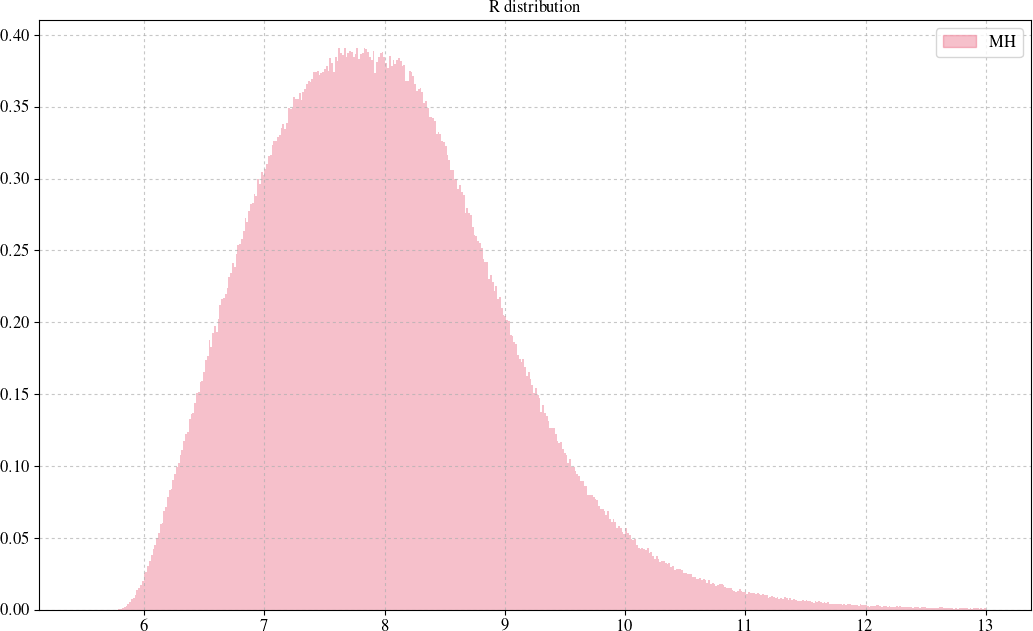
\includegraphics[width=0.5\textwidth, height=5cm]{../pictures/r_bound_distribution.png} \\ 
	\vspace{0.2cm}
	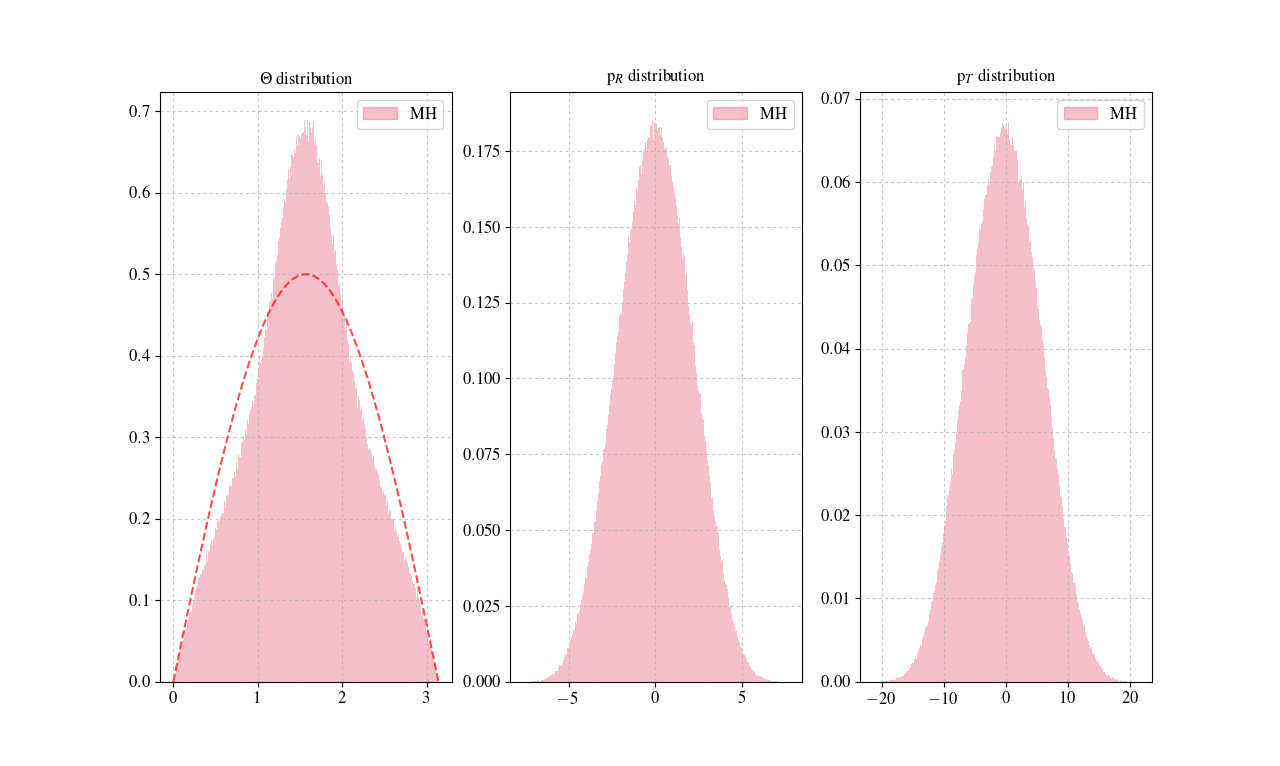
\includegraphics[width=0.8\textwidth, height=6cm]{../pictures/theta_bound_distribution.png} \\
	\vspace{0.2cm}
	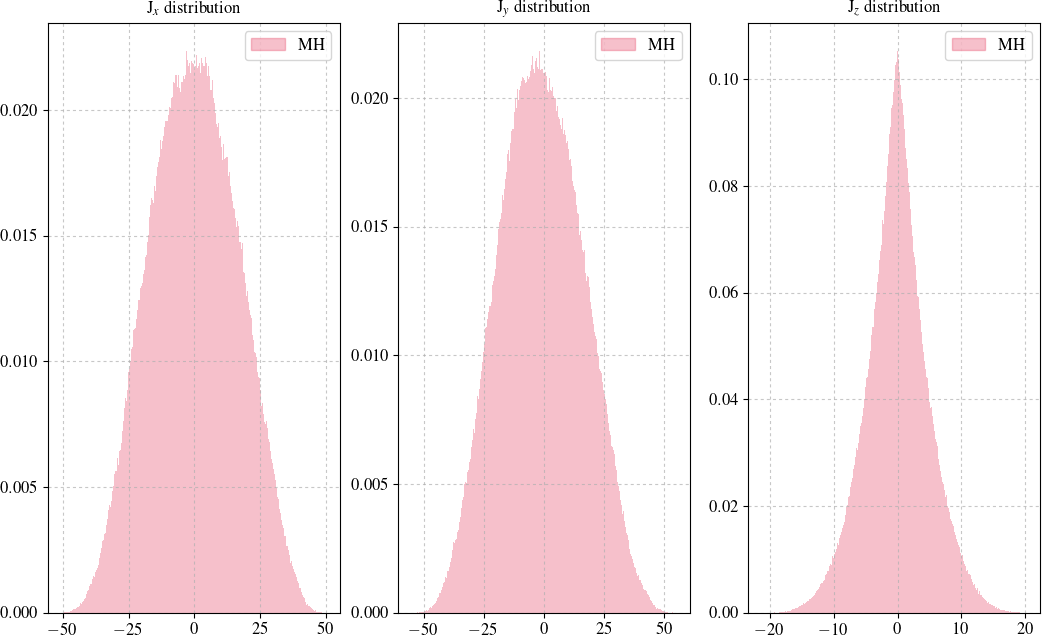
\includegraphics[width=0.7\textwidth, height=6cm]{../pictures/j_bound_distribution.png} 
\caption{Распределения переменных $R$, (\textbf{первый ряд}), $\Theta$, $p_R$, $p_T$ (\textbf{второй ряд}), $J_x$, $J_y$, $J_z$ (\textbf{третий ряд}) для связанных состояний CO$_2-$Ar при $T = 300 K$, полученные модифицированным методом MH, 2.000.000 точек}
	\label{fig:bound}
\end{figure}

